\subsection{Interessentanalyse}
Dette afsnit vil undersøge hvilke interessenter der er, og hvilken interesse de har i problemet og en eventuel løsning af problemet. Vi har udvalgt fem interessenter ud fra emnet lamper, da belysning fra lamper er det centrale i det initierende problem. Formålet med interessentanalysen er at finde ud af hvilke interessenter som denne rapport vil løse problemet for. De fem interessenter er: designer, producent, butik, kunde og bruger, som vist på nedenstående figur.



\begin{figure}[H]
	\centering
  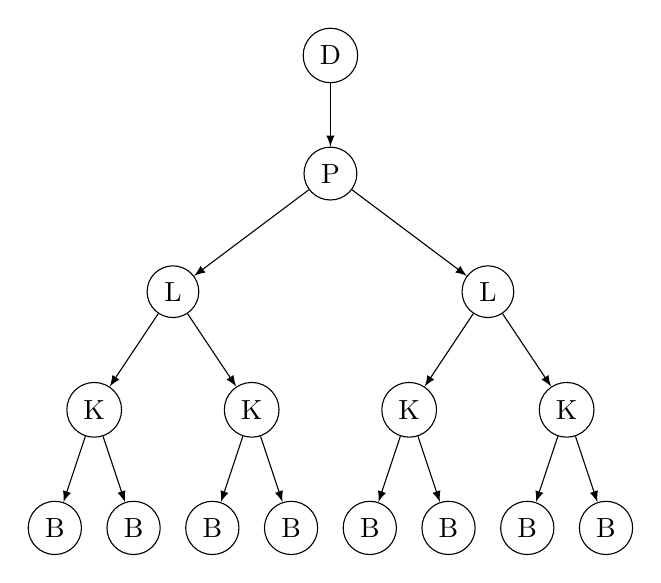
\begin{tikzpicture}[
    level 1/.style={sibling distance=40mm},
    level 3/.style={sibling distance=20mm},
    level 4/.style={sibling distance=10mm},
    every node/.style={draw,circle},
    arrow/.style={edge from parent/.style={draw,-latex}}
  ]
  \node {D}
      child[arrow] { node{P}
          child { node{L}
              child { node{K}
                  child {node{B}}
                  child {node{B}}
              }
              child { node{K}
                  child {node{B}}
                  child {node{B}}
              }
          }
          child { node{L}
              child { node{K}
                  child {node{B}}
                  child {node{B}}
              }
              child { node{K}
                  child {node{B}}
                  child {node{B}}
              }
          }
      }
  ;
  \end{tikzpicture}
  \caption{Viser princippet bag, hvordan lampen overføres mellem de fem interessenter designer(D), producent(P), lampebutik(L), kunde(K) og bruger(B).}
  \label{fig:interessenter}
\end{figure}
% Sælgeren bliver også indirekte ramt, hvis mange kunder henvender sig fordi de gerne vil have en lampe returneret og byttet, så kræver det ressourcer fra lampebutikkers side. Derfor vil det også være til lampebutikkers fordel, at en kunde vil være i stand til at købe "den rigtige" lampe første gang eller en lampe, der er lidt dyrere fordi den giver den ønskede effekt.

\subsubsection{Designere}
Designere er interesseret i at deres design bliver solgt og er derfor sandsynligvis interesseret i et program, der kan hjælpe dem med at gøre deres design mere populært.

 
Vi har haft kontakt med to forskellige lampedesignere, danske Erik Mortensen, og svenske David Wahl fra IKEA. Erik Mortensen sagde: 
\begin{center}
\textit{"I alle mine lamper er valg af lyskilde og placering sket på grundlag af test via prototyper. De fleste af mine lamper er prototyper"}.

\textit{"Jeg har i en del år arbejdet med lampedesign. og har derfor mest været optaget af armaturets/lampens skulpturelle udtryk, men da det jo er en lampe skal den selvfølgelig  også opfylde det belysningsmæssige."} Mailen kan ses i bilag \ref{sec:mailErik}.
\end{center}

På baggrund af dette kan man altså uddrage at Erik Mortensen udelukkende benytter sig af prototyper, til at visualisere lampens lys på.

David Wahl sagde:
\begin{center}
\textit{"Apart from hand sketching and physical prototypes, we use the 3D modeling application Solid Works in IKEA of Sweden. And for renderings we use either the built in renderer, or photo works, which is also part of solid works."} Mailen kan ses i bilag \ref{sec:mailDavid}.
\end{center}

David Wahl bruger altså, ligesom Erik Mortensen, prototyper, men derudover benytter han sig også af computerprogrammet Solid Works.

Designerne har interesse i at få visualiseringsproblemet løst, da det kan have økonomiske konsekvenser for dem, hvis en bruger er utilfreds med en lampes lys, der kan få kunden til at returnere varen. Dette kan betyde færre solgte lamper, som sandsynligvis kan gøre at en designers design ikke er så meget værd som før.

\subsubsection{Producenter}
Producenten samarbejder med designeren om at udvikle lampen. Producentens rolle er at fremstille lampen på baggrund af designet. Når lamperne er produceret sendes de ud til lampebutikkerne. Producenten kan have en interesse i, at kunderne køber deres produkter i lampebutikkerne, da der er mulighed for, at dette vil medføre at lampebutikkerne bestiller flere af deres produkter hjem. Vi har haft kontakt med en belysningskonsulent, som her ønsker at være anonym. Belysningskonsulenten sagde følgende om producenternes interesse i problemet:

\begin{center}
\textit{"Det er blevet en kompliceret proces at producere en lampe ift. EU lovgivning i dag så jeg har svært ved at se at producenterne vil koste endnu flere penge til produkter til privatmarkedet som måske kun køber en lampe til 3000 kr. som ofte kun interesserer sig for den laveste pris og ikke den bedste service og rådgivning. Så producenters incitament til ligge investeringer hos privatkunder er meget begrænset."} - Mailen kan ses i bilag \ref{sec:mailbelysning}. 
\end{center}

Belysningskonsulenten mener altså at producenterne ikke vil smide en masse penge ind i privatmarkedet, da det ikke gavner dem økonomisk. 

Producenterne får sandsynligvis flere midler til større produktion af en given lampe, hvis lampen er populær. desto flere solgte lamper til en lampebutik, desto flere penge tjener producenten. Det er derfor et problem for producenterne, hvis en lampe returneres, grundet en utilfreds kunde. Dog er producenterne, som nævnt i citatet fra belysningskonsulenten, ikke nødvendigvis interesseret i at investere penge i rådgivning, og dermed også visualisering af en lampe og dens belysning for kunder. I stedet er dette en opgave, som i større grad ligger hos lampebutikken, som beskrevet i næste afsnit.


\subsubsection{Lampebutikker}
Lampebutikken er interesseret i at sælge flest mulige lamper, da dette giver større indkomst for butikken. Derudover er butikken også interesseret i, at kunden køber den 'rigtige' lampe første gang, da butikken på denne måde undgår utilfredse kunder, som vil returnere lamperne.


\subsubsection{Kunder}
Kunden er interesseret i at visualisere hvordan lys udbreder sig fra en lampe, da dette vil hjælpe kunden med at afgøre hvordan lampen passer ind i en kontekst, og kunden kan derfor undgå fejlkøb. Dette er kunden interesseret i, da det i sidste ende vil gavne brugeren af lampen, hvis kunden er i stand til at købe en lampe, som passer ind i konteksten. Kundens interesse i visualisering af lampen og dens belysning underbygges af følgende citat fra den førnævnte belysningskonsulent:
\begin{center}
\textit{"Der er overraskende mange der gerne vil se lyset inden de køber lamper."} Mailen kan ses i bilag \ref{sec:mailbelysning} 
\end{center}

Kundernes interesse vil også være at undgå de økonomiske konsekvenser, hvis der købes en lampe, som opfylder de forventninger, som kunden forestillede at lampen opfyldte, men først indses efter lampen er installeret og emballagen er brudt, og lampen dermed ikke kan returneres.

\subsubsection{Brugere}
Det er brugerne der i sidste ende benytter sig af lamperne i deres hjem eller på deres arbejde. Dette gør brugerne til den gruppe af interessenter, som påvirkes direkte af problemet, da de må leve med konsekvenserne, som belysningen fra en lampe kan medføre, som omtalt i afsnit \ref{sec:konsekvenser}. Et eksempel på brugere, er hjemme i privaten, hvor der kan være mange forskellige typer lamper, som skal passe ind i hjemmet. Hvis en person i hjemmet bruger en lampe, som har en belysning, der ikke passer ind i hjemmet pga.\ manglende visualisering ved købet, vil dette påvirke brugerne i hjemmet, da dårlig belysning kan have sundhedsmæssige konsekvenser som omtalt i afsnit \ref{sec:konsekvenser}.



\subsubsection{Målgruppen}
Som beskrevet i forrige afsnit, er det både designere, producenter, butikker, kunder og brugere, der påvirkes af problemet. Det er nu relevant at afgøre hvem problemløsningen retter sig mod, da dette danner grundlag for, hvordan løsningen skal udvikles og hvem der kan indrages i løsningen og udarbejdelsen af løsningsforslaget.

Som illustreret på figur \ref{fig:interessenter} er det lampebutikkerne, som har den direkte kontakt til kunderne og via kunderne en forbindelse til brugerne. Designere er fravalgt, da vi ud fra mails fra Wahl og Mortensen kan uddrage, at de allerede har værktøjer til at visualisere lys fra lamper, og som der ses på skitsen har designeren ikke nogle direkte kontakt til kunden eller brugeren. Man kunne forestille sig, at problemet kunne løses allerede fra producentens side. Ud fra udtagelsen fra belysningskonsulenten, er vi dog blevet informeret om, at producenterne ikke er interesseret i at bruge ressourcer på at løse problemet, da det ikke gavner producenterne direkte. Derudover er det ikke producentens opgave at vejlede kunder til det bedste køb af lamper, dette er derimod lampebutikkens opgave.

Hvis man retter problemløsningen mod lampebutikker, og laver en løsning der gør det muligt for kunder at visualisere lamperne bedre, er det sandsynligt at kunderne vil være mere tilfredse med deres lamper, da de har mulighed for at se lampens belysning inden købet. For lampebutikker kan dette betyde, at kunden ikke returnerer lige så mange lamper, og dette vil bidrage til øget kundetilfredshed, som i sidste ende gavner både lampebutikker og kunderne. Hvis kunden er i stand til at købe en lampe som passer ind i den korrekte kontekst vil dette også tilfredsstille brugeren. 

\subsubsection*{Opsummering}
I afsnittet er der blevet argumenteret for, at det påvirker brugeren af lampen hvis kunden ikke kan visualisere hvordan lyset udspreder sig fra en lampe, og dette vil i sidste ende også påvirke lampebutikkerne. Derudover er der blevet argumenteret for, at det er mest fordelagtigt at rette løsningen mod lampebutikker, da dette også løser problemet for brugerne.

Dette afsnit er relevant i forhold til den senere problemformulering, da der er blevet argumenteret for hvem det er, som har problemet, samt hvilken målgruppe det senere produkt skal udvikles til.
